\documentclass[a4paper,slidestop,xcolor=pst,blue]{beamer}

\input{slidesHeader.tex}

\title[Capa de Persistencia]{Capa de Persistencia}

\author[P. S{\'a}nchez]{\alert{Pablo S{\'a}nchez}}

\institute[IIE]{
		   Dpto. Ingenier{\'i}a Inform{\'a}tica y Electr{\'o}nica \\
		   Universidad de Cantabria \\
		   Santander (Cantabria, Espa{\~n}a) \\
		   \texttt{p.sanchez@unican.es}
}

\date{}

\begin{document}

\begin{frame}[c]
	\titlepage
	\begin{columns}
		\column{0.50\linewidth}
			\centering
    		\includegraphics[width=.28\textwidth,keepaspectratio=true]{images/istr.eps}
		\column{0.50\linewidth}
			\centering
			\includegraphics[width=.25\textwidth,keepaspectratio=true]{images/uc.eps}
	\end{columns}
\end{frame}

\begin{frame}[c]
    \frametitle{\alert{Advertencia}}
    \begin{center}
        Todo el material contenido en este documento no constituye en modo alguno una obra de referencia o apuntes oficiales mediante el cual se puedan preparar las pruebas evaluables necesarias para superar la asignatura. \ \\
        \ \\
        Este documento contiene exclusivamente una serie de diapositivas cuyo objetivo es servir de complemento visual a las actividades realizadas en el aula para la transmisi{\'o}n del contenido sobre el cual versar{\'a}n las mencionadas pruebas evaluables.  \ \\
        \ \\
        Dicho de forma m{\'a}s clara, \alert{estas transparencias no son apuntes y su objetivo no es servir para que el alumno pueda preparar la asignatura.}
    \end{center}
\end{frame}

\section{Introducción}

\subsection{Objetivos y Bibliografía}

\begin{frame}[c]
    \frametitle{Objetivos del Tema}
    \begin{enumerate}[<+->]
         \item Comprender en profundidad cuáles son las responsabilidades de la capa de persistencia.
         \item Comprender el funcionamiento de los puentes de persistencia de objetos.
         \item Conocer los patrones de persistencia estructurales.
         \item Conocer los patrones de acceso a datos.
         \item Conocer los patrones de control de la concurrencia.
         \item Ser capaz de utilizar JPA para generar esquemas relacionales.
         \item Ser capaz de utilizar repositorios para acceder a datos persistentes.
    \end{enumerate}
\end{frame}

\begin{frame}[c]
    \frametitle{Bibliografía}
    \begin{thebibliography}{1}

        \bibitem[Fowler, 2002]{Fowler2002}
        Fowler, M. (2002).
        \newblock {\em {Patterns of Enterprise Application Architecture}}.
        \newblock Addison-Wesley.

        \bibitem[Esposito and Saltarello, 2014]{Esposito2014}
        Esposito, D. y Saltarello, A. (2014).
        \newblock {\em {Microsoft .NET - Architecting Applications for the
          Enterprise}}. 2ª Ed..
        \newblock Microsoft Press

        \bibitem[Bauer, 2015]{Bauer2015}
        Bauer, C., King. G. y Gregory G. (2015).
        \newblock {\em {Java Persistence with Hibernate}}. 2ª Ed.
        \newblock Manning

        %% JPA

        %% Spring Data

    \end{thebibliography}
\end{frame}

\subsection{Contexto: Capa de Persistencia}

\begin{frame}
    \frametitle{Capa de Persistencia}
    \only<1|handout:2>{
        \rput[lt](0,0){
            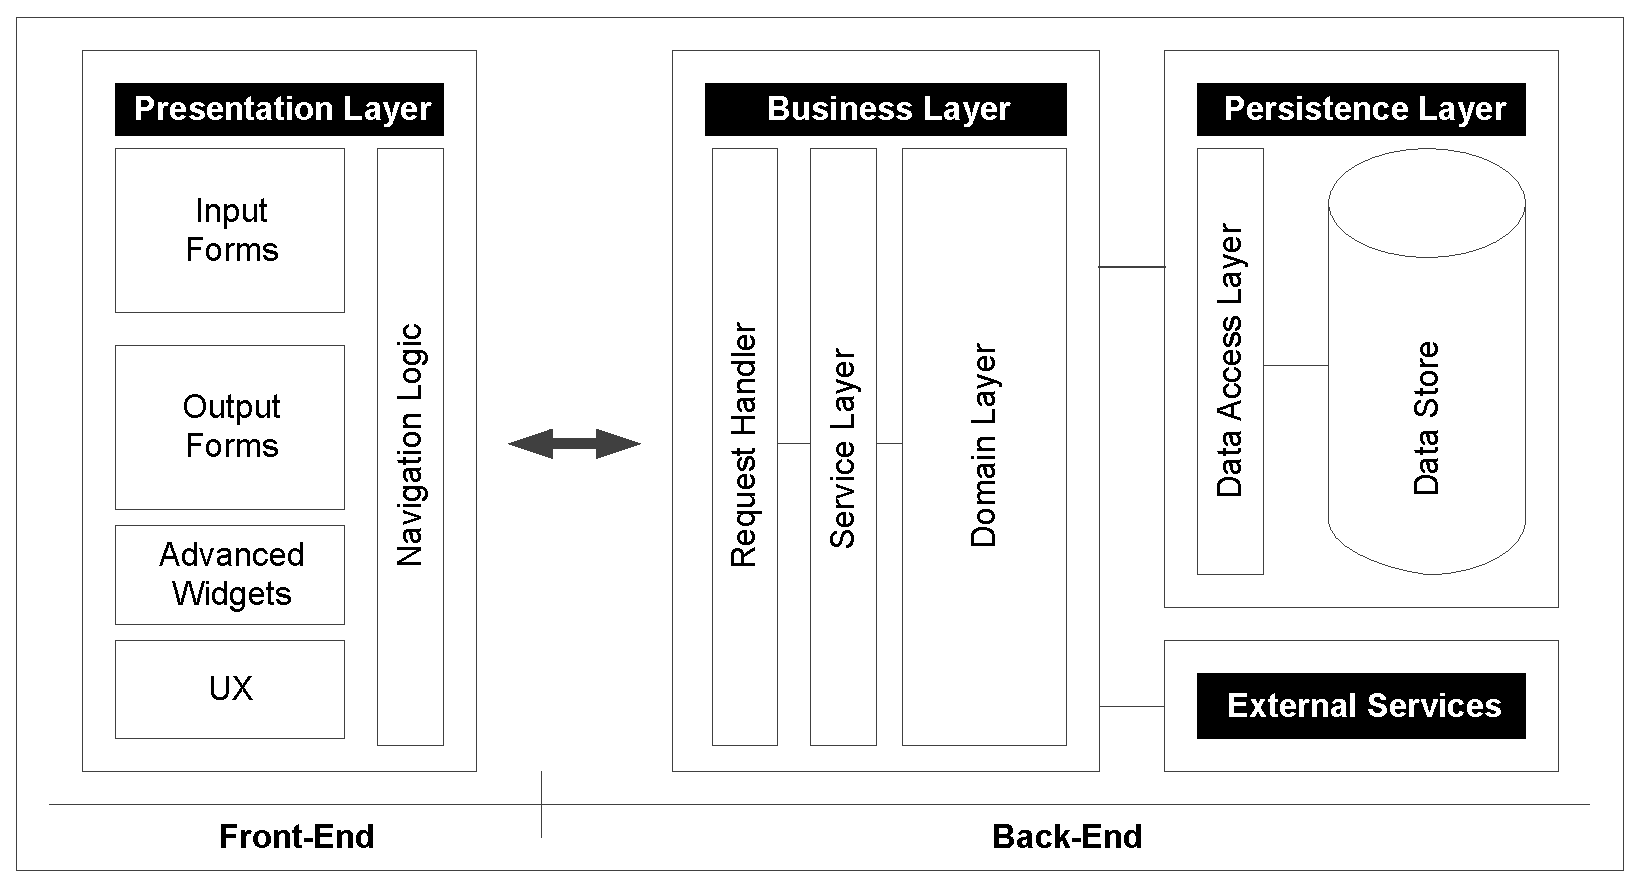
\includegraphics[width=\linewidth]{images/intro/enterpriseArchitectures00.eps}
        }
    }
    \only<2|handout:2>{
        \rput[lt](0,0){
            \includegraphics[width=\linewidth]{images/intro/enterpriseArchitectures01.eps}
        }
    }
\end{frame}

\begin{frame}[c]
	\frametitle{Responsabilidades de la Capa de Persistencia}
	\begin{enumerate}[<+->]
        \item Almacenar los datos de manera no volátil.
        \item Recuperar datos del almacén persistente,
        \item Asegurar la disponibilidad de los datos.
        \item Controlar la integridad de los datos.
        \item Asegurar un acceso eficiente a los datos.
	\end{enumerate}
\end{frame}

\begin{frame}[c]
    \frametitle{Tecnologías de Persistencia}
    \begin{description}[<+->]
        \item[Relacional] Madurez, robustez y propiedades ACID.
        \item[NoSQL] Escalabilidad y rendimiento sacrificando ACID.
        \item[XML/JSON] Simplicidad.
    \end{description}
\end{frame}

\section{Puentes de Persistencia de Objetos}

\subsection{Impedancia Objeto - Persistencia}

\begin{frame}[c]
    \frametitle{Impedancia Objeto - Persistencia}
    \begin{block}{Impedancia Objetual}
    La \emph{impedancia objetual} se refiere al desacoplamiento que puede existir en los conceptos del paradigma orientado a objetos y el paradigma utilizado por el almacén de persistencia.
    \end{block}
\end{frame}

\begin{frame}[c]
    \frametitle{Impedancia Objeto - Relacional}
    \begin{center}
        \includegraphics[width=\linewidth]{images/ooMismatch/ooMismatch00.eps}
    \end{center}
\end{frame}

\begin{frame}[c]
    \frametitle{Impedancia Objeto - Relacional}
    \begin{center}
        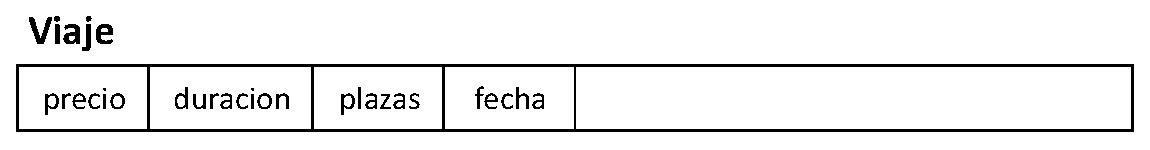
\includegraphics[width=0.8\linewidth]{images/ooMismatch/ooMismatch01.eps}
    \end{center}
\end{frame}

\begin{frame}[c]
    \frametitle{Impedancia OR: Claves Primarias}
    \begin{center}
        \includegraphics[width=\linewidth]{images/ooMismatch/ooMismatch09.eps}
    \end{center}
\end{frame}

\begin{frame}[c]
    \frametitle{Impedancia OR: Granularidad}
    \begin{center}
        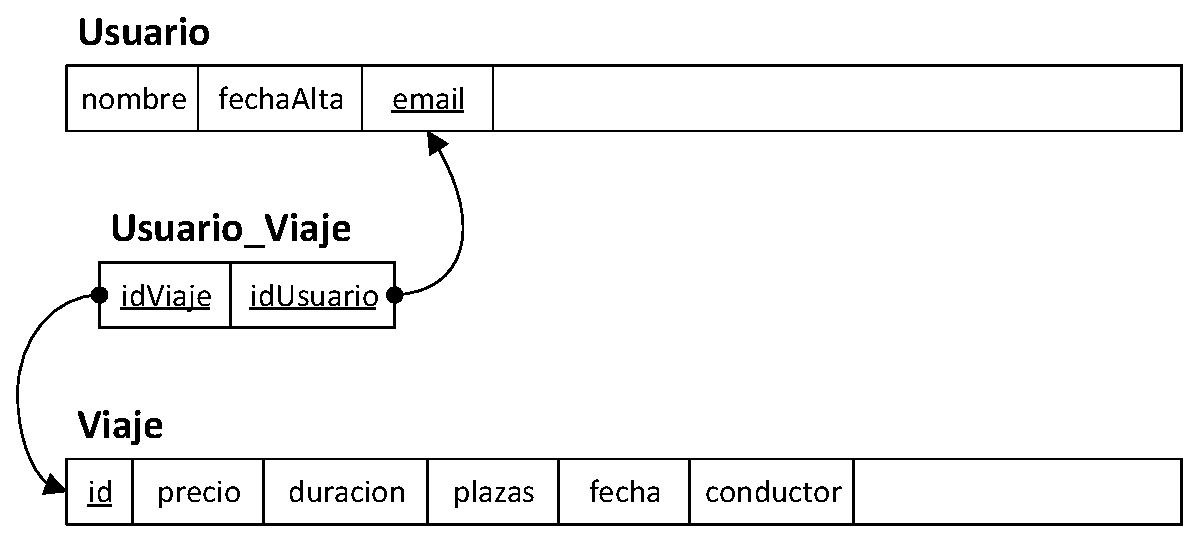
\includegraphics[width=0.8\linewidth]{images/ooMismatch/ooMismatch08.eps}
    \end{center}
\end{frame}

\begin{frame}[c]
    \frametitle{Impedancia OR: Atributos Multivaluados}
    \begin{center}
        \includegraphics[width=\linewidth]{images/ooMismatch/ooMismatch02.eps}
    \end{center}
\end{frame}

\begin{frame}[c]
    \frametitle{Impedancia OR: Atributos Multivaluados}
    \begin{center}
        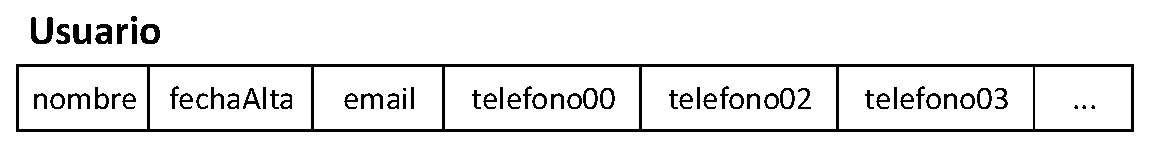
\includegraphics[width=0.8\linewidth]{images/ooMismatch/ooMismatch03.eps}
    \end{center}
\end{frame}

\begin{frame}[c]
    \frametitle{Impedancia OR: Herencia}
    \begin{center}
        \includegraphics[width=\linewidth]{images/ooMismatch/ooMismatch04.eps}
    \end{center}
\end{frame}

\begin{frame}[c]
    \frametitle{Impedancia OR: Navegabilidad Asociaciones}
    \begin{center}
        \includegraphics[width=\linewidth]{images/ooMismatch/ooMismatch05.eps}
    \end{center}
\end{frame}

\begin{frame}[c]
    \frametitle{Impedancia OR: Navegabilidad Asociaciones}
    \begin{center}
        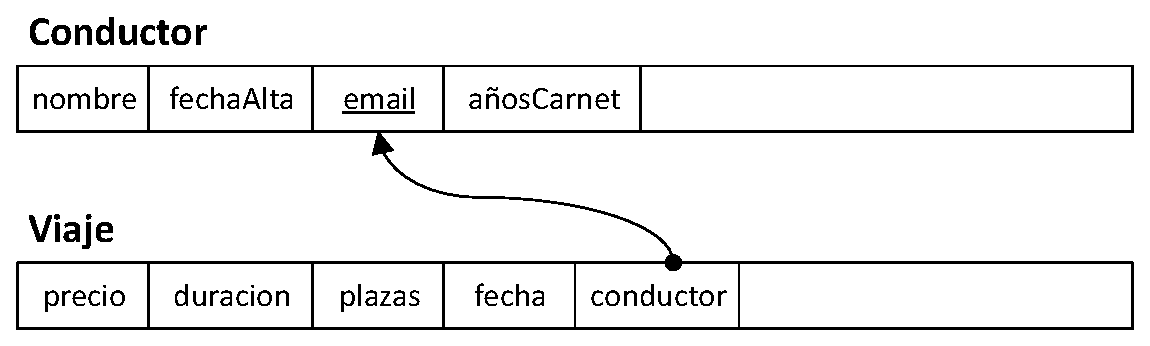
\includegraphics[width=0.8\linewidth]{images/ooMismatch/ooMismatch06.eps}
    \end{center}
\end{frame}

\begin{frame}[c]
    \frametitle{Impedancia OR: Asociaciones Muchos a Muchos}
    \begin{center}
        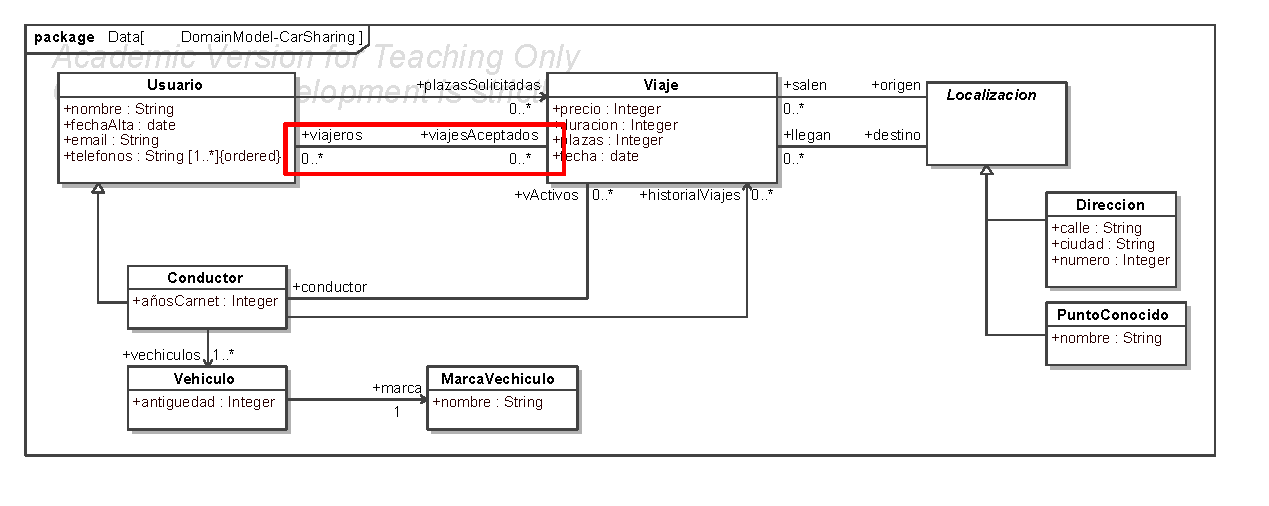
\includegraphics[width=\linewidth]{images/ooMismatch/ooMismatch07.eps}
    \end{center}
\end{frame}

\begin{frame}[c]
    \frametitle{Impedancia OR: Asociaciones Muchos a Muchos}
    \begin{center}
        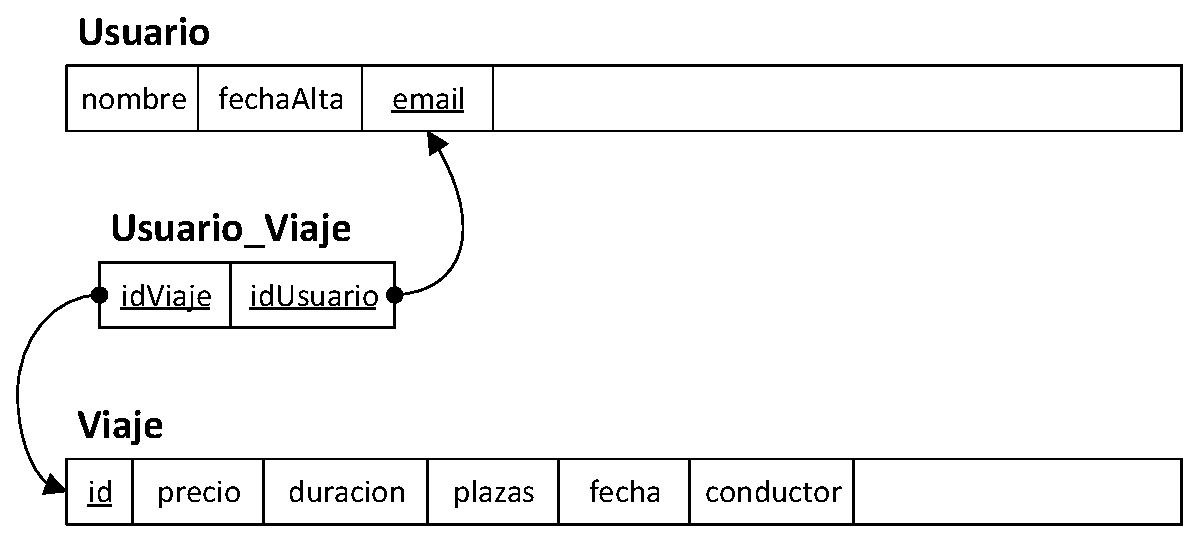
\includegraphics[width=0.8\linewidth]{images/ooMismatch/ooMismatch08.eps}
    \end{center}
\end{frame}

\subsection{Esquema Puentes Objeto-Persistencia}

\begin{frame}
    \frametitle{Puentes de Persistencia de Objetos}
    \only<1|handout:3>{
        \rput[lt](0,0){
            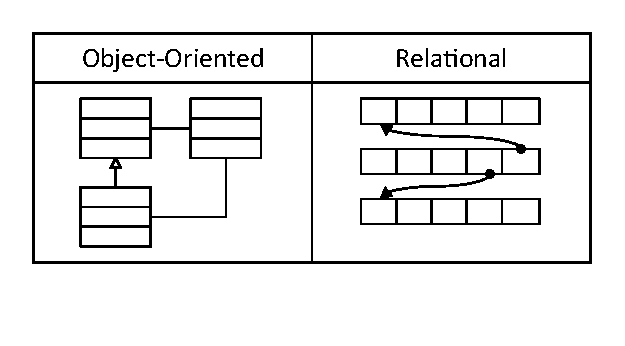
\includegraphics[width=\linewidth]{images/ooMismatch/orm00.eps}
        }
    }
    \only<2|handout:3>{
        \rput[lt](0,0){
            \includegraphics[width=\linewidth]{images/ooMismatch/orm01.eps}
        }
    }
    \only<3|handout:3>{
        \rput[lt](0,0){
            \includegraphics[width=\linewidth]{images/ooMismatch/orm02.eps}
        }
    }
    \only<4|handout:3>{
        \rput[lt](0,0){
            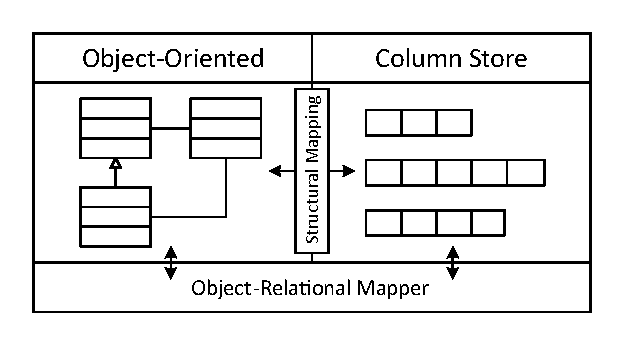
\includegraphics[width=\linewidth]{images/ooMismatch/orm03.eps}
        }
    }
\end{frame}

\section{Patrones Estructurales}

\subsection{Conceptos Básicos}

\subsubsection{Class to Table}

\begin{frame}[c]
    \frametitle{Class to Table}
    \begin{block}{Problema}
        \begin{enumerate}
            \item ¿Cómo transformo una clase a relacional?
        \end{enumerate}
    \end{block}
    \uncover<2->{
        \begin{block}{Solución}
            Si la clase es una \emph{entidad}, no está afectada por herencia, y no tiene atributos compuestos:
            \begin{enumerate}
                \item<3-> Crear una tabla con el mismo nombre de la clase.
                \item<4-> Crear una columna en dicha tabla por cada atributo de la clase.
                \item<5-> Asignar como tipo de la columna el tipo que corresponda a cada atributo.
            \end{enumerate}
        \end{block}
    }
\end{frame}

\begin{frame}
    \frametitle{Class to Table}
    \rput[lt](3,0){
            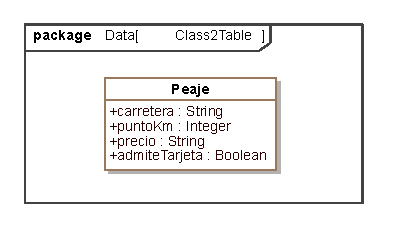
\includegraphics[width=0.60\linewidth]{images/structure/class2Table00.eps}
    }
    \only<2->{
        \rput[lt](2.5,-4.5){
                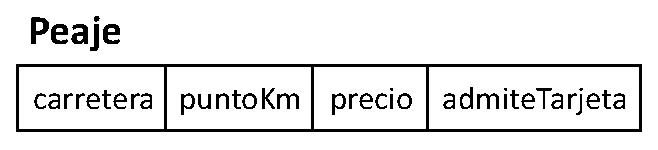
\includegraphics[width=0.60\linewidth]{images/structure/class2Table01.eps}
        }
    }
\end{frame}


\subsubsection{Identity Field}

\begin{frame}[c]
    \frametitle{Identity Field}
    \begin{block}{Problema}
        \begin{enumerate}
            \item ¿Cómo determino la clave primaria de cada objeto que necesito guardar en la base de datos relacional?
        \end{enumerate}
    \end{block}
    \uncover<2->{
        \begin{block}{Característica de una Buena Clave}
            \begin{enumerate}
                \item<2-> Única para cada objeto.
                \item<3-> Inmutable (o cuasi inmutable).
                \item<4-> Fácil de comparar.
            \end{enumerate}
        \end{block}
    }
\end{frame}

\begin{frame}[c]
    \frametitle{Identity Field - Claves en el Modelo Relacional}
    \begin{center}
        \includegraphics[width=0.60\linewidth]{images/structure/identityField00.eps}
    \end{center}
\end{frame}

\begin{frame}[c]
    \frametitle{Identity Field - Solución}
    \begin{block}{Solución}
        Dada una clase $A$:
        \begin{enumerate}[<+->]
            \item<2-> Utilizar un atributo o conjunto de atributos ya existentes en esa clase $A$ que ya sean clave o puedan desempeñar adecuadamente el papel de clave.
            \item<3-> Añadir un nuevo atributo a la clase $A$ que ejerza el papel de clave primaria para su almacenamiento en una base de datos relacional. En este caso, dicho atributo no se deberá utilizar más allá de la capa de persistencia.
        \end{enumerate}
    \end{block}
\end{frame}

\begin{frame}[c]
    \frametitle{Identity Field - Ejemplo}
    \begin{center}
        %% Clase viaje con nuevo atributo introducido.
        \includegraphics[width=0.60\linewidth]{images/structure/identityField01.eps}
    \end{center}
\end{frame}

\begin{frame}[c]
    \frametitle{Identity Field - Estrategias de Generación de Claves}
    \begin{enumerate}
        \item<1-> Autogenerada por el gestor de bases de datos.
            \begin{itemize}
                \item<2-> Necesitas salvar el objeto para conocer su clave.
                \item<3-> Limita ciertas optimizaciones a nivel de ORM.
            \end{itemize}
        \item<2-> Autogenerada por la aplicación.
        \item<3->
    \end{enumerate}
\end{frame}

\subsection{Transformación de Asociaciones}

\subsubsection{Embedded Value}

\subsubsection{Foreign Key Mapping}

\subsection{Transformación de Herencias}

\subsubsection{Association Table Mapping}

\subsubsection{Single Table Inheritance}

\subsubsection{Class Table Inheritance}

\section{Patrones de Acceso a Datos}

\subsubsection{Data Access Object}

\begin{frame}[c]
    \frametitle{Data Access Objects - Data Mappers}
    \begin{block}{Problema}
        Hacer que los objetos de un modelo de dominio puedan ser almacenados en, y recuperados de, un elemento persistente, \uncover<2->{manteniendo a la vez dichos objetos independientes de la tecnología concreta utilizada para su persistencia;}
        \uncover<3->{de manera que los cambios que se produzcan en dicho almacén persistente no afecten al modelo de dominio}.
    \end{block}
    \uncover<4->{
        \begin{block}{Solución}
            Por cada clase del modelo del dominio, crear una clase, denominada \emph{Data Access Object (DAO)} o \emph{Data Mapper}, que se encargue de gestionar el almacenamiento y recuperación de los objetos de dicha clase mediante una tecnología de persistencia concreta.
        \end{block}
    }
\end{frame}

\begin{frame}[c]
    \frametitle{Data Mapper - Ejemplo}
    \begin{center}
        TODO
        %% Ejemplo de clase con su correspondiente Data Mapper
        %% Enlace a repositorio de GitHub conteniendo un ejemplo de Data Mapper
        %% \includegraphics[width=0.60\linewidth]{images/structure/identityField01.eps}
    \end{center}
\end{frame}

%% Complicaciones:
%% * Actualización de modificaciones.
%% * Actualización de colecciones.
%% * Cómo cargar un objeto con sus relaciones sin traerme todo la base de datos a memoria.

%% Ventajas:
%%
%% * Aisla el modelo de dominio de la tecnología de persistencia.
%% * Permite intercambiar capas de persistencia para testing.
%% * Permite hybrid polystores.
%% * Permite optimizaciones en persistencia sin modificar dominio.
%% *

\subsubsection{Inheritance Mappers}

\subsubsection{Metadata Mapping}

\subsubsection{Repositories}

\begin{frame}[c]
    \frametitle{Repository}
    \begin{block}{Problema}
        Cómo manipular colecciones de objetos como si estuviesen alojados en memoria, de manera independiente a la tecnología de persistencia utilizada,
    \end{block}
    \uncover<4->{
        \begin{block}{Solución}
            Por cada colección de objetos de la cual haya que extraer un cierto subconjunto, crear
        \end{block}
    }
\end{frame}


\subsection{Patrones Auxiliares}

\subsubsection{Lazy Load}

\subsubsection{Identity Field}

\subsubsection{Query Object}

\subsubsection{Unit of Work}

\begin{frame}[c]
    \frametitle{Unit of Work}
    \begin{block}{Problema}
        Cómo manipular colecciones de objetos como si estuviesen alojados en memoria, de manera independiente a la tecnología de persistencia utilizada,
    \end{block}
    \uncover<4->{
        \begin{block}{Solución}
            Por cada colección de objetos de la cual haya que extraer un cierto subconjunto, crear
        \end{block}
    }
\end{frame}

\section{Patrones de Control de la Concurrencia}

\subsection{Pessimistic Lock}

\subsection{Optimistic Lock}

\section{Java Persistence API}

\subsection{Elementos Estructurales}

\subsection{Validación}

\subsection{Comportamiento}

\begin{frame}[c]
    \frametitle{Entity Manager}
    %% Unidad de Trabajo en JPA
\end{frame}

\begin{frame}[c]
    \frametitle{Ciclo de Vida de una Entidad JPA}
    %% Diagrama de las actividades
    %% Se puede llegar a través de agregados, es decir, como referencia desde
    %% una entidad, normalmente un agregado
\end{frame}




\begin{frame}[c]
    \frametitle{Ciclo de Vida de una Entidad JPA}
    %% Detecta transacciones de usuario.
\end{frame}

\section{Spring Data}

\section{Sumario y Conclusiones}

\end{document}
